\section{System Architecture}
\label{sec:arch}
The platform connects task-level reasoning to production-scoped execution
through three component groups (Fig.~\ref{fig:arch}). Team and strategy
services maintain channels, members, tasks, messages, memory, and replaceable
engine adapters. Governance services resolve capabilities, limits, approval,
dispatch, confirmation, and intervention records. Industrial integration
converts semantic DAQ/DCW operations into protocol I/O. These groups share
line--product--recipe--run context and linked evidence stores. Registration
services, a typed SDK, and REST, MCP, agent-to-agent, CLI, and console
interfaces provide sanctioned extension points. Figure~\ref{fig:arch} groups these
cooperating responsibilities rather than imposing one execution sequence
on every operation.

The architecture separates three state objects with complementary roles.
A task states the intended outcome and its responsible member. Production
objects identify the configured definition and active execution context.
Execution records state what was admitted, sent, confirmed, and observed.
Shared identifiers join these objects for inspection. An agent engine can
therefore be replaced without redefining a recipe or a driver's evidence
contract. The project is distributed under Apache-2.0; repository links are
withheld for anonymous review.

\begin{figure*}[!t]
\centering
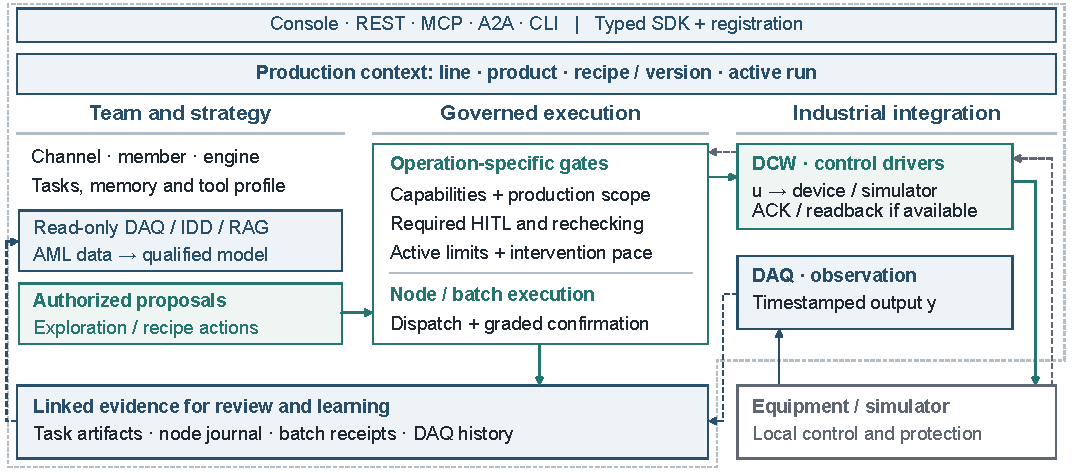
\includegraphics[width=\textwidth]{resources/fig-architecture-2026.pdf}
\caption{Component architecture of the governed supervisory framework.
Team and strategy services propose actions; governance services resolve
authority and execution checks; industrial integration separates control
$u$ from acquisition $y$. Production context and linked evidence connect
these responsibilities. Equipment protection and fast regulation operate
outside the platform boundary.}
\label{fig:arch}
\end{figure*}

\subsection{Semantic Nodes and Production Context}
DAQ nodes expose engineering quantities with units, precision, timestamps,
and quality metadata. Their contracts cover scalars, vector profiles, image
frames, and mirrored manufacturing-execution-system (MES) records. MES
integration supports mirrored acquisition and direct endpoint mappings.
DCW nodes describe writable engineering quantities and their driver
configuration. Drivers own serialization, transport handling, and available
readback; platform services own authority and admission. Thus a proposal can
name holding pressure in bar while the driver supplies the corresponding
OPC UA, register, topic, or REST representation.

Implemented protocol families include Modbus TCP, Modbus RTU-over-TCP,
OPC UA, MQTT, and HTTP/REST, with MES REST mappings. Q1 exercises simulator
writes over Modbus TCP, OPC UA, MQTT, and HTTP; RTU-over-TCP is
acquisition-only. The admission ablation uses a separate mock driver.
DAQ acquisition uses per-node cadences and a rotating sweep. Timestamped
history supplies decisions, exports, and response queries independently of
the agent's reasoning duration.

Lines associate equipment with an active product, recipe, and run. Recipe
definitions are versioned; a running batch retains its execution context,
so saving a definition and applying it are separate operations. This
distinction supports a practical progression: investigate a candidate,
observe its result, save the accepted parameterization, and apply the
selected version to a run. Acquisition samples and dispatch receipts can
then be interpreted against the production context in which they arose.

An onboarding blueprint declares devices, signal maps, units, roles, and
initial setpoints. A differential ensure pass creates missing objects and
reconciles declared configuration drift. Connecting another process changes
this blueprint and its process-specific objective, guards, and proposal
policy while reusing the execution services. This is the reuse boundary
exercised across the process missions.
\label{sec:reuse}

\subsection{Capabilities and Channel Profiles}
A channel organizes a job and its collaborating members; persisted
capabilities authorize industrial operations. Node bindings define readable
or controlled node scope and execution mode, while recipe capabilities
define an authorized production scope. The server also restricts tools by
channel profile. These two checks answer complementary questions: whether
this class of job may invoke an operation, and whether this particular
member may perform it on the selected production objects.

In the current v0.7.66 implementation, observation channels perform
acquisition, analysis, and knowledge work, while Auto Modeling Lab (AML)
training channels prepare datasets and models. Both have read-only plant
access. AML-optimization channels invoke \texttt{optimization\_explore}
with control and target-scope validation. Operational channels use
authorized recipe operations. Direct public \texttt{dcw\_control} and
\texttt{dcw\_rollback} are closed; sanctioned platform workflows reach the
internal governed node executor. Consequently, a written task instruction
or retrieved document cannot expand the industrial tool surface.

This decomposition supports collaboration through explicit artifacts. An
observation member can deliver a diagnostic report, a training member can
deliver an evaluated model reference, and an optimization member can use
authorized evidence to propose a bounded intervention. Each receiving
member operates under its own channel profile and capability checks. Team
coordination transfers information while execution authority remains
attached to the actor and production scope.

\subsection{Analysis, Models, and Candidate Proposals}
The information path begins with timestamped acquisition and production
context. A merged DAQ export aligns selected signals for industrial data
diagnostics (IDD); diagnostic reports describe the observed operating
regime. Retrieval-augmented generation (RAG) supplies relevant process
knowledge and prior reports for interpretation. These outputs inform the
strategy's choice of controls, targets, and stopping criteria. Write
authority is resolved independently when the candidate reaches execution.

AML provides a separate data-to-model path. Its dataset builder selects
line--product--recipe-scoped histories, cleans samples by state and range,
aligns them to a sampling grid, and constructs windows within runs.
Run-based partitions and training-partition normalization produce a
dataset manifest, tensors, and a cleaning report. These artifacts identify
the controls, targets, features, runs, and transformations presented to
training. The asynchronous production training route invokes Python,
exports an Open Neural Network Exchange (ONNX) artifact, evaluates it, and
applies gates before candidate registration. Registry stages distinguish
candidate, shadow, production, and retired models; promotion carries its
own approval workflow.

Model binding and eligibility checks govern model-assisted tools, including
declared uncertainty, out-of-distribution, and physics information. Current
lineage enforcement is primarily line-scoped. Each production training job
retains its exported model, evaluation report, and gate decision as
identifiable artifacts. Bounded exploration also operates without a model.
A trained model, a candidate proposal, and an industrial command thus remain
distinct outputs. The evaluation below focuses on execution contracts;
model-assisted control--response is not evaluated.

\subsection{Two Execution Lifecycles}
\label{sec:tasklifecycle}
Figure~\ref{fig:runtime} separates the current runtime routes. Bounded
optimization exploration validates the writable node and target ownership,
then invokes the internal governed executor. It associates a single-factor
control intervention with target observations. Operational recipe work
uses \texttt{recipe\_trial} for a candidate override without saving a
version, \texttt{recipe\_update} for a new definition,
\texttt{recipe\_apply} for dispatch, and \texttt{recipe\_rollback} for
version restoration. Restoring a definition and commanding the equipment
are separately evidenced operations.

In Q6, an approved holding-pressure trial links its receipt to the next
quality observation; a later recipe update retains the accepted parameters.

Persistence follows the route. A successful changed-value node write opens
a node-optimization record before the observation wait. Bounded exploration
then waits, queries the target, and saves a separate exploration summary.
Recipe dispatch instead creates a batch run with per-parameter receipts;
its caller performs the subsequent wait, observation, and decision. Saving
an accepted parameterization requires a separate recipe update. These
distinct records preserve the correspondence between an operation and its
evidence. Section~\ref{sec:eval} identifies each experiment's tested interface.
